% FD analysis chapter -- using shower reconstruction to distinguish pi0s and electrons?
% Target: 10 pages

\graphicspath{{FarDetectorAnalysis/Figs/}}

%----------------------------------------------------------------------------------------------------------------------------------------------------------------------------
%\chapter{Electron Reconstruction for $\nu_e$ Oscillation Signal at the DUNE Far Detector}\label{chap:FDAnalysis}
\chapter{The $\nu_e$ Oscillation Signal at the DUNE Far Detector}\label{chap:FDAnalysis}

A primary aim of the DUNE experiment, as discussed in Chapter~\ref{chap:DUNE}, is to make precision measurements of the PMNS matrix parameters describing neutrino oscillations by searching for electron neutrino appearance from the predominantly muon neutrino beam (i.e. $\nu_{\mu} \rightarrow \nu_e$ oscillation, described by Equation~\ref{eq:ElectronNeutrinoAppearance}).  This channel is of critical importance for all oscillation-related physics and thus requires very efficient reconstruction and selection.  Methods developed to provide reconstruction of these events were discussed in detail in Chapter~\ref{chap:LArTPCReconstruction} and utilised in this present chapter in the selection of simulated charged-current (CC) $\nu_e$ events ($\nu_e$CC) in the DUNE far detector.

The selection presented in the following sections represents the very first generation analysis for the DUNE experiment and serves primarily to demonstrate the principle of selecting these events in a large LArTPC.\footnote{This work was undertaken with Dominic Brailsford (Lancaster University), who was working on the complementary $\nu_{\mu}$CC selection.}  Much work is needed to advance the analysis to comply with DUNE requirements and many improvements may be expected as further developments progress.  It should also be noted the reconstruction discussed in Chapter~\ref{chap:LArTPCReconstruction} is not the only solution and various other techiniques, primarily using the Pandora toolkit \cite{Pandora2015}, have been assessed, notably in Section~\ref{sec:FDCut}.  The selection presented in Section~\ref{sec:FDMVA} does utilise the novel reconstruction detailed in this thesis however, due to significant recent progress, it is likely the selection will continue to explore all reconstructions in LArSoft and take advantage of the continuing developments.  This outlook will be briefly discussed in Section~\ref{sec:FDOutlook}.

%----------------------------------------------------------------------------------------------------------------------------------------------------------------------------
\section{Cut-Based Tuning}\label{sec:FDCut}

This section details the early developments of a selection which utilises only Pandora reconstruction and a cut-based approach.  This procedure shows promise at performing as well as the more established multi-variate analysis (MVA) method, discussed in Section~\ref{sec:FDMVA}, but is used here mainly to tune the selection.

As will be discussed in Section~\ref{sec:FDMVA}, the current MVA implementation of the $\nu_e$CC selection contains a mixture of particle level and event level variables and requires significant understanding before developments may progress.  The motivation behind considering a simplified selection is to facilitate a careful evaluation of the events and the analysis utilises a distinct particle identification (PID) system to perform particle level discrimination, separate from the event level classification.  As with the majority of this present chapter, this work is very preliminary and represents the first studies into these areas for the DUNE experiment.

%----------------------------------------------------------------------------------------------------------------------------------------------------------------------------
\subsection{Selection}\label{sec:FDCutSelection}

The elementary cut-based selection utilises Pandora reconstruction for tracks and showers and an MVA approach to PID for each of the reconstructed objects.  This PID framework \cite{GrantPID2016} utilises variables such as ratios of deposited charge, conicalness, average dE/dx and dE/dx ratios to form a hypothesis for each of the particle types muon, electron, proton, photon, pion.  The selection simply selects events which contain candidate electron showers and places a cut on the value of the electron-MVA result to attempt to identify the electrons.  The separation between electrons and photons for the electron-MVA value of the highest energy shower in each event is demonstrated in Figure~\ref{fig:ElectronMVA}.  It is immediately evident that, given the strengths of LArTPC techonology to separate these showering particle types, significant progress is required in the next decade.

\begin{figure}
  \centering
  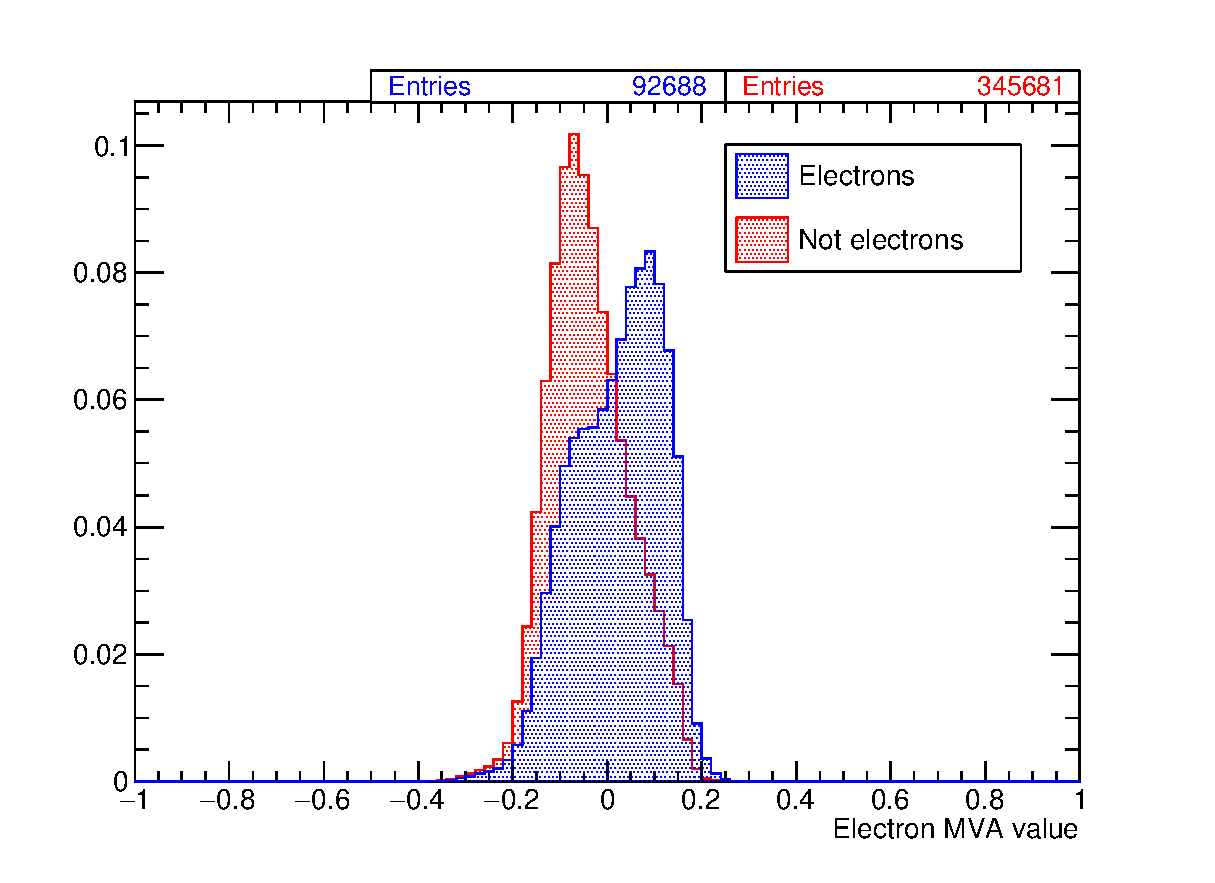
\includegraphics[width=10cm]{ElectronMVA.eps}
  \caption[The output of a multi-variate approach to particle identification when attemping to identify electrons.]{The output of a multi-variate approach to particle identification when attemping to identify electrons.}
  \label{fig:ElectronMVA}
\end{figure}

To tune this cut, and for further tunings discussed in Section~\ref{sec:FDCutFV}, a physics-based approach was taken.  Arguably the most important consequence of this analysis is to search for CP-violation, so the tuning was designed to maximise the capability of this.  For each electron-MVA value, the $\nu_e$-appearance energy spectrum was determined for the CP-conservation ($\delta_{CP}=0$) and CP-violation ($\delta_{CP}=\pi/2$) hypotheses and maximising the $\chi^2$ between the distributions ensures the greatest discriminating ability of the analysis to discern hints of CP-violation.  This is demonstrated in Figure~\ref{fig:ElectronMVATune}, and a cut value of 0.02 is found to provide the best differentiation.  The events were POT-weighted (protons on target) and the oscillation probabilities were provided by the Prob3++ framework \cite{Prob3++}.

\begin{figure}
  \centering
  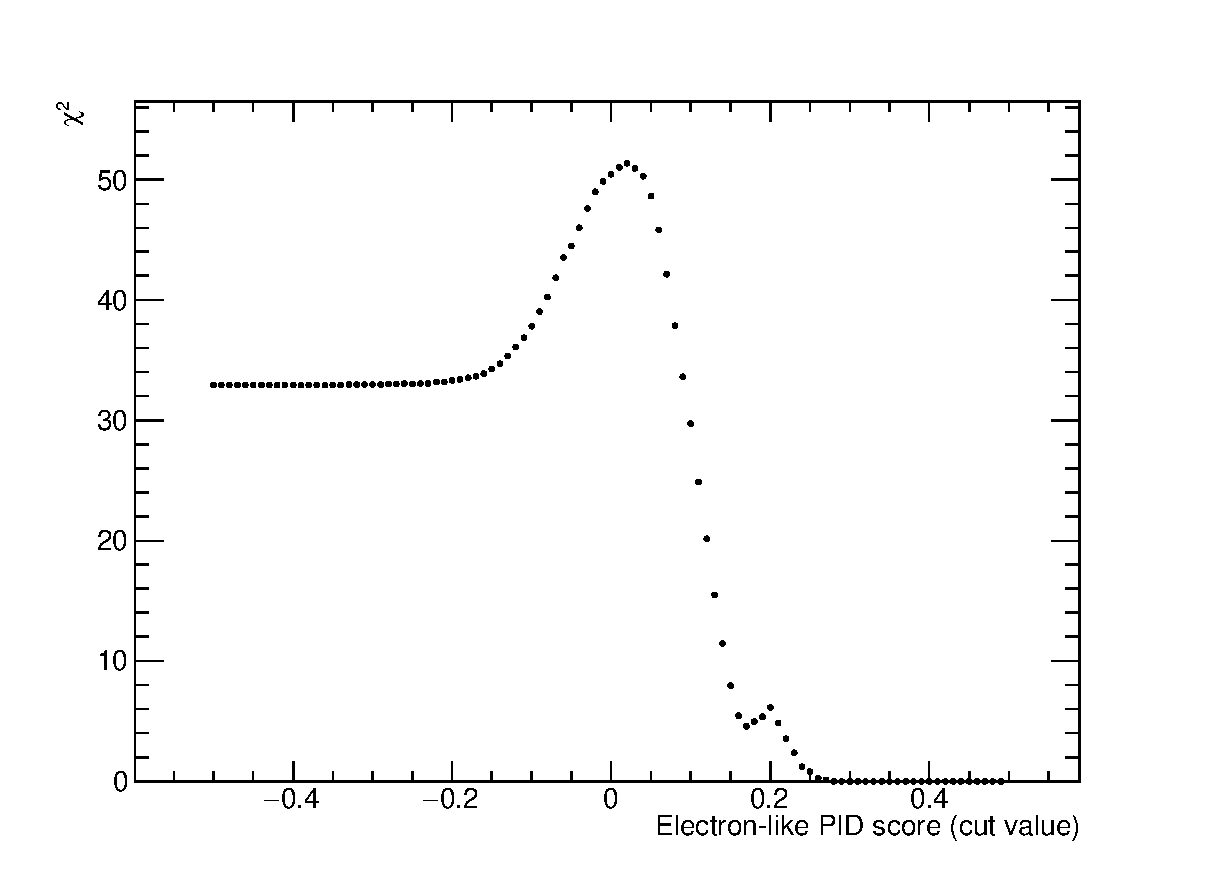
\includegraphics[width=10cm]{ElectronMVATune.eps}
  \caption[The process of tuning the electron cut in the simple cut-based selection by maximising the effect of CP-violation on the oscillation probabilities.]{The process of tuning the electron cut in the simple cut-based selection by maximising the effect of CP-violation on the oscillation probabilities.}
  \label{fig:ElectronMVATune}
\end{figure}

The efficiency and purity of the selection with just this simple cut is demonstrated in Figure~\ref{fig:FDCutEffPur}.  It is found the selection already looks reasonable and, as will be observed in Section~\ref{sec:FDMVA}, is competitative to the MVA-based analysis.

\begin{figure}
  \centering
  \begin{subfigure}[t]{0.48\linewidth}
    \centering
    \caption{}
    \label{fig:FDCutEff}
  \end{subfigure}
  \hfill
  \begin{subfigure}[t]{0.48\linewidth}
    \centering
    \caption{}
    \label{fig:FDCutPur}
  \end{subfigure}
  \caption{}
  \label{fig:FDCutEffPur}
\end{figure}

%----------------------------------------------------------------------------------------------------------------------------------------------------------------------------
\subsection{Fiducial Volume Tuning}\label{sec:FDCutFV}

A similar approach to the tuning described in the previous section may be utilised to optimise the fiducial volume (FV) applied in the selection.  This has not previously been performed in the DUNE far detector, with estimations and assumptions applied during the development of the analysis.  The distance of the start point of the electron shower from the walls of the cryostat is considered over a range of energies and oscillation probabilities, as before, and the $\chi^2$ between the distributions for maximum CP-conservation and CP-violation maximised to provide the optimal parameters.

Example plots showing the tuning of the $x$-coordinate are the subject of Figure~\ref{fig:FDFVTune}.  The tuned FD coordinates, along with the cryostat dimensions, are shown in Table~\ref{tab:FV}.

%----------------------------------------------------------------------------------------------------------------------------------------------------------------------------
\section{MVA-Based Selection}\label{sec:FDMVA}

%----------------------------------------------------------------------------------------------------------------------------------------------------------------------------
\subsection{MVA Input Variables}\label{sec:FDMVAVariables}

%----------------------------------------------------------------------------------------------------------------------------------------------------------------------------
\subsection{Analysis Performance}\label{sec:FDMVAPerformance}

%----------------------------------------------------------------------------------------------------------------------------------------------------------------------------
\section{Outlook for Future Selections}\label{sec:FDOutlook}
